\chapter{Algorytm rankingowy}

\section{Idea algorytmu rankingowego}

Przedstawiona w~rozdziale drugim koncepcja średniej Bayesa została wykorzystana do stworzenia wzoru, pozwalającego obliczyć przydatność recenzji. Dzięki niej użytkownik może w~łatwy sposób odfiltrować treści ocenione przez innych użytkowników jako nieprzydatne i~zapoznać się z~rzetelną recenzją interesującego go produktu. System umożliwia bowiem sortowanie recenzji wg ich przydatności. Własność ta budowana jest przede wszystkim na podstawie głosów oddanych przez użytkowników systemu, którzy zapoznając się z~recenzją, mają możliwość oznaczenia jej jako przydatna lub nie.

Nie jest to jednak jedyne zastosowanie przydatności recenzji w~systemie\linebreak RevCommunity. Ma ona bowiem także wpływ na wagę oceny recenzji w~ostatecznej ocenie produktu. Każdy z~produktów w~systemie może posiadać wiele recenzji, a~każda z~nich zawiera subiektywną ocenę opisywanego produktu nadaną przez jej autora. Obliczanie łącznej oceny produktu jako średniej arytmetycznej ocen wynikających z~recenzji może prowadzić do uzyskania oceny, która nie oddaje we właściwy sposób faktycznej wartości produktu. Możliwa jest bowiem sytuacja, w~której produkt zostanie oceniony przez nierzetelnych użytkowników, którzy z~różnych przyczyn, np. będąc pracownikami konkurencyjnego producenta, będą zabiegali o~celowe zaniżenie oceny produktu. Aby uniknąć wspomnianej sytuacji, w~celu obliczenia ostatecznej oceny, zastosowano średnią ważoną ocen pochodzących z~recenzji danego produktu, gdzie wagami są przydatności recenzji. Dzięki temu wiarygodne recenzje, napisane przez rzetelnych użytkowników, mają większą wagę, a~co za tym idzie, większy wpływ na ocenę produktu.

Wzór pozwalający na obliczenie przydatności recenzji R ma następującą postać:

\begin{equation}
\bar{x_{R}}=\frac{w_{m}Cm+w_{g}\frac{p}{p+n}(p+n)+w_{a}\frac{p_{a}}{p_{a}+n_{a}}(p_{a}+n_{a})}{w_{m}C+w_{g}(p+n)+w_{a}(p_{a}+n_{a})}*100\%
\end{equation}
gdzie:\\
m - domyślna przydatność recenzji, czyli średnia arytmetyczna przydatności wszystkich recenzji w~systemie\\
C - stała dobrana eksperymentalnie\\
p - liczba głosów pozytywnych oddanych na recenzję R\\
n - liczba głosów negatywnych oddanych na recenzję R\\
$p_{a}$ - liczba głosów pozytywnych oddanych na wszystkie recenzje autora recenzji R\\
$n_{a}$ - liczba głosów negatywnych oddanych na wszystkie recenzje autora recenzji R\\
$w_{m}$ - waga domyślnej przydatności recenzji\\
$w_{g}$ - waga głosów oddanych na recenzję R\\
$w_{a}$ - waga głosów oddanych na wszystkie recenzje autora recenzji R.\\


Podstawowym składnikiem przedstawionego wzoru są głosy oddane przez użytkowników systemu. Zostały one przedstawione jako iloczyn stosunku liczby głosów pozytywnych do wszystkich oddanych na daną recenzję i~łącznej liczby głosów. Wyrażenie $\frac{p}{p+n}$ odpowiada wartości $x$, natomiast $(p + n)$, wartości $n$ w~definicji średniej Bayesa przedstawionej w~punkcie \ref{sec:algTeotia}.

Przydatność recenzji nie zależy jednak tylko od głosów oddanych przez użytkowników. Jednym z~dodatkowych czynników jest domyślna przydatność recenzji, będąca średnią arytmetyczną przydatności wszystkich recenzji w~systemie. Wartość ta odpowiada wartości domyślnej $m$ w~przedstawionej wcześniej koncepcji średniej Bayesa i~również występuje wraz ze stałą wartością $C$, która została dobrana eksperymentalnie.

Ostatnim czynnikiem wpływającym na użyteczność recenzji jest ocena autora, wyrażona jako iloczyn stosunku liczby głosów pozytywnych do wszystkich oddanych na recenzje danego użytkownika oraz łącznej liczby głosów oddanych na jego recenzje. Obecność oceny autora we wzorze jest zabezpieczeniem systemu przed zalewem treści sponsorowanych. Publikujący je użytkownik otrzyma negatywne głosy, które obniżą jego ocenę, dzięki czemu przydatność wszystkich jego recenzji również zostanie zmniejszona. Tym samym istnieje mniejsze prawdopodobieństwo, że dotrą one do użytkownika końcowego, poszukującego rzetelnych informacji o~produkcie. 

Wszystkim wspomnianym czynnikom składającym się na przydatność recenzji zostały dodatkowo przypisane wagi, tak aby można było kontrolować ich wpływ na obliczaną wartość.

Warto zauważyć, że przytoczony wzór można łatwo zredukować do prostszej postaci:

\begin{equation}\label{eq:przydatnosc}
\bar{x_{R}}=\frac{w_{m}Cm+w_{g}{p}+w_{a}p_{a}}{w_{m}C+w_{g}(p+n)+w_{a}(p_{a}+n_{a})}*100\%
\end{equation}\\

Uproszczona w~ten sposób formuła została zaimplementowana w~aplikacji\linebreak RevCommunity.

Kolejną wartością, której obliczanie bazuje na koncepcji średniej Bayesa, jest ranga recenzenta. Dzięki niej użytkownik uzyskuje poglądową informację o~ogólnej jakości wszystkich recenzji napisanych przez użytkownika. Wartość ta obliczana jest według przedstawionego poniżej wzoru:

\begin{equation}\label{eq:ocUzyt}
\bar{x_{U}}=\frac{w_{ma}C_{a}m_{a}+w_{a}p_{a}}{w_{ma}C_{a}+w_{g}(p+n)+w_{a}(p_{a}+n_{a})}*100\%
\end{equation}
gdzie:\\
$m_{a}$ - domyślna ocena użytkownika, równa 0,5\\
$C_{a}$ - stała dobrana eksperymentalnie\\
$p_{a}$ - liczba głosów pozytywnych oddanych na wszystkie recenzje autora recenzji R\\
$n_{a}$ - liczba głosów negatywnych oddanych na wszystkie recenzje autora recenzji R\\
$w_{ma}$ - waga domyślnej oceny użytkownika\\
$w_{a}$ - waga głosów oddanych na recenzje autora recenzji R\\

Wyliczona w~ten sposób ocena użytkownika mapowana jest na jedną z~dostępnych rang, zależnie od jej wartości. Tabela \ref{tab:rangi} przedstawia rangi dostępne w~systemie wraz z~odpowiadającymi im zakresami wartości oceny użytkownika wyliczonej za pomocą wzoru \ref{eq:ocUzyt}.

\begin{table}[H]
\centering
\begin{tabular}{|c||c|}  
\hline
\textbf{Ranga} & \textbf{Wartość [\%]} \\
\hline\hline
\textbf{Niekompetentny} & 0-20 \\  
\hline
\textbf{Niezaufany} & 20-40 \\  
\hline
\textbf{Przeciętny} & 40-60 \\  
\hline
\textbf{Godny zaufania} & 60-80 \\  
\hline
\textbf{Ekspert} & 80-100 \\  
\hline
\end{tabular}
\caption{Rangi użytkowników}\label{tab:rangi}
\end{table}


\section{Opis eksperymentów}

\subsection{Przygotowanie danych i~symulacja}

W celu weryfikacji stworzonej koncepcji algorytmu rankingowego zbudowana została aplikacja symulująca proces oceniania recenzji. Model danych aplikacji testowej jest uproszony względem systemu RevCommunity i~obejmuje tylko użytkowników i~recenzje. 

Każdy z~użytkowników posiada zbiór recenzji swojego autorstwa, liczbę recenzji, które oceni w~trakcie symulacji, a~także wartość procentową określającą  domyślne prawdopodobieństwo otrzymania pozytywnego głosu przez recenzję jego autorstwa. Dodatkowo każdy z~użytkowników może zostać oznaczony jako oszust, co spowoduje, że w~trakcie głosowania będzie oceniał dobre recenzje jako złe i~odwrotnie. Użytkownicy - oszuści mają za zadanie symulować obecnych w~realnym świecie użytkowników sponsorowanych.

Recenzje posiadają natomiast unikatowy identyfikator, liczbę uzyskanych głosów pozytywnych i~negatywnych, przydatność, autora, a~także prawdopodobieństwo otrzymania pozytywnego głosu, które jest liczbą losową z~zakresu [90\% x ; 110\% x], gdzie x to domyślne prawdopodobieństwo otrzymania pozytywnego głosu, przypisane do autora recenzji. Należy dodatkowo zaznaczyć, że wylosowane prawdopodobieństwo jest zawsze liczbą z~zakresu [0;1]

Ważną rolę w~programie testowym odgrywają także parametry pozwalające sterować przebiegiem symulacji. Wszystkie dostępne ustawienia deklarowane są w~klasie Parameters, która definiuje jednocześnie ich domyślne wartości. Na jej podstawie budowane są kolejne zbiory parametrów przydatne dla poszczególnych testów, nadpisujące tylko niezbędne wartości. Najważniejsze parametry, które można dostosować w~opisywanej aplikacji testowej to:

\begin{itemize}
\item Wagi oraz wartości stałe wykorzystywane podczas obliczania przydatności recenzji i~oceny autora,
\item Liczba użytkowników biorących udział w~symulacji,
\item Procentowy udział użytkowników - oszustów,
\item Liczba recenzji biorących udział w~symulacji.
\end{itemize}


Wykonanie symulacji wymaga wcześniejszego wygenerowania kolekcji użytkowników i~recenzji. W celu lepszego odwzorowania rzeczywistości użytkownicy zostają podzieleni na trzy grupy: przeciętnych, aktywnych i~biernych. Użytkownikowi należącemu do odpowiedniej grupy przypisywana jest następnie liczba recenzji, które oceni on podczas symulacji. Średnia liczba recenzji, przypadająca na użytkownika, określana jest za pomocą stałej wartości, pochodzącej ze zbioru parametrów i~odpowiada ona liczbie recenzji ocenianych przez przeciętnych użytkowników. Aktywni użytkownicy  mają natomiast przyporządkowaną losową wartość, większą od średniej, a~użytkownicy bierni mniejszą. Następnie, spośród wszystkich użytkowników, losowana jest określona przez parametry liczba oszustów. Ostatnim elementem procesu jest wylosowanie użytkowników będących autorami recenzji. Każdemu z~nich przyporządkowywane jest domyślne prawdopodobieństwo otrzymania pozytywnego głosu. Kolejnym etapem jest proces generowania recenzji, w~którym każdej z~nich przyporządkowywany jest losowy autor, a~także losowane jest prawdopodobieństwo otrzymania pozytywnego głosu.

Po wygenerowaniu niezbędnych obiektów następuje symulacja oceniania recenzji przez użytkowników. Pierwszym etapem procesu jest wylosowanie dla każdego użytkownika określonej liczby recenzji, które oceni w~czasie symulacji. Następnie, dla każdej z~nich, losowana jest wartość z~zakresu [0;1], która jeśli okaże się większa lub równa prawdopodobieństwu otrzymania pozytywnego głosu, powoduje zwiększenie licznika głosów negatywnych recenzji. W przeciwnym wypadku inkrementowany jest licznik głosów pozytywnych. Sytuacja wygląda inaczej, jeżeli oceniający jest oszustem. Wtedy wylosowanie liczby większej niż przypisane recenzji prawdopodobieństwo skutkuje dodaniem głosu pozytywnego. 

Ostatecznie, dla każdej recenzji wyliczana jest przydatność przy wykorzystaniu wzoru \ref{eq:przydatnosc} i~przygotowywany jest specyficzny dla danego testu raport.

\subsection{Test I - przegląd danych}

Pierwszy z~zaproponowanych testów umożliwia pełny podgląd systemu po przeprowadzeniu symulacji. Jego kod źródłowy znajduje się w~klasie DefaultTest. Dzięki niemu możemy podejrzeć podstawowe informacje, takie jak wagi użyte do obliczania przydatności czy średnią użyteczność w~systemie, ale również szczegółowe dane dotyczące recenzji i~recenzentów. Dla recenzji są to kolejno:

\begin{itemize}
\item identyfikator,
\item prawdopodobieństwo otrzymania pozytywnego głosu, będące jednocześnie oczekiwaną wartością przydatności,
\item liczbę oddanych głosów,
\item liczbę głosów pozytywnych,
\item stosunek głosów pozytywnych do wszystkich,
\item przydatność,
\item błąd, czyli różnica między przydatnością oczekiwaną a~uzyskaną, podniesiona do kwadratu.
\end{itemize}

Dane użytkowników reprezentowane są przez:

\begin{itemize}
\item identyfikator,
\item liczbę głosów oddanych na recenzje użytkownika,
\item liczbę głosów pozytywnych,
\item ocenę użytkownika,
\item identyfikatory recenzji należących do użytkownika.
\end{itemize}

Całkowity przegląd danych okazał się szczególnie przydatny w~ustalaniu odpowiednich wag i~wartości stałych biorących udział w~obliczaniu przydatności recenzji i~oceny autora.

Wartości błędów wykorzystane są do obliczenia RMSE (ang. \textit{root mean squared error}), który pozwala na szybkie porównanie różnych przypadków testowych. RMSE mierzy o~ile jednostek średnio różnią się wartości obliczone od wartości domyślnej.\cite{rmseWiki}\\
\begin{equation}
RMSE=\sqrt{\frac{\sum_{t=1}^n (\bar{y_{t}}-y_{t})^2}{n}}
\end{equation}
gdzie:\\
n- liczba pomiarów\\
$\bar{y_{t}}$ - wartość domyślna\\
$y_{t}$ - wartość uzyskana\\

\subsection{Test II - Badanie wpływu liczby głosów na błąd przydatności}

Kolejny test, którego kod źródłowy znajduje się w~klasie ProgressiveTest, posłużył do zbadania zależności pomiędzy liczbą użytkowników, która przekłada się na liczbę oddanych głosów, a~różnicą pomiędzy spodziewaną i~uzyskaną wartością przydatności, wyrażoną w~postaci RMSE. Intuicja podpowiada, że im więcej głosów oddano na recenzję, tym jej przydatność jest bardziej wiarygodna, a~tym samym błąd powinien być mniejszy. Aby sprawdzić czy wspomniana zależność jest zachowana, przygotowano test, w~którym symulacja powtarzana jest kilkakrotnie, za każdym razem dla innej liczby użytkowników. Przed wykonaniem testu istnieje możliwość ustawienia początkowej i~końcowej wartości tego parametru, a~także wartości o~jaką parametr ten będzie zwiększany w~każdej iteracji. Liczba recenzji dla każdej iteracji pozostaje stała.

Poniżej przedstawiono raport uzyskany po wykonaniu testu dla 100 recenzji i~wzrastającej liczby użytkowników z~zakresu od 30 do 300. Nagłówek zawiera wartość stałą i~wagi wykorzystane do obliczenia przydatności recenzji. Poniżej znajdują informacje o~każdej z~iteracji. Pierwsza kolumna informuje o~liczbie użytkowników. Kolejna zawiera błąd w~postaci RMSE, natomiast ostatnia średnią liczbę głosów przypadających na recenzję. Poniżej przedstawiono również wykres stworzony na podstawie raportu. Obrazuje on wpływ wzrostu liczby użytkowników na wartość RMSE.

\begin{lstlisting}
defaultUsefulnessWeight: 1
reviewRateWeight: 8
authorRateWeight: 3
const: 15

users	RMSE	votes/review	
30	0.05942	8.93
60	0.05217	12.83
90	0.04425	18.09
120	0.0424	24.76
150	0.04169	32.71
180	0.03963	40.35
210	0.03967	47.47
240	0.03859	55.32
270	0.03554	62.94
300	0.03585	70.78
\end{lstlisting}

\begin{figure}[h]
	\centering
	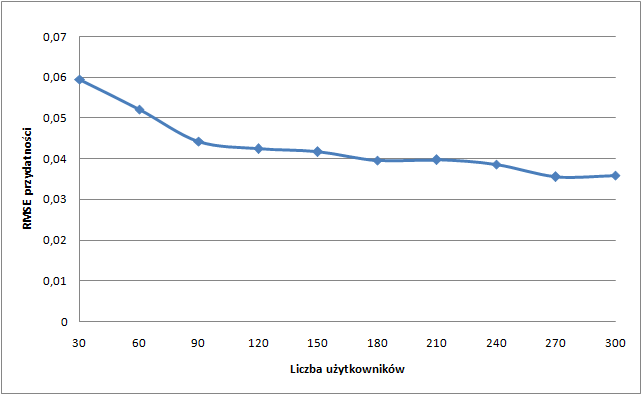
\includegraphics[width=\textwidth, keepaspectratio=true]{images/ProgressiveTest.png}
	\caption{Liczba użytkowników a~pierwiastek błędu średniokwadratowego przydatności recenzji}
\end{figure}

Analizując uzyskane dane, można zauważyć, że wzrost liczby użytkowników, a~co za tym idzie, głosów oddanych na recenzje, istotnie powoduje spadek błędu. Innymi słowy, recenzje posiadające więcej głosów posiadają użyteczność bliższą wartości oczekiwanej. Dzieje się tak, ponieważ wraz ze wzrostem liczby głosów oddanych na recenzję, rośnie ich wpływ na wartość wyliczanej użyteczności. Dla małej liczby głosów, użyteczność recenzji normalizowana jest przez wartość domyślnej użyteczności.

\subsection{Test III - Badanie odporności systemu na obecność użytkowników - oszustów}

Ostatni z~testów dotyczy odporności systemu na obecność użytkowników - oszustów. Jego kod źródłowy znajduje się w~pliku LiarsTest.java. Głównym celem testu jest sprawdzenie jak zmienia się wartość błędu wraz ze wzrostem liczby użytkowników sponsorowanych w~systemie. Podobnie jak w~poprzednim teście, kolejne symulacje przeprowadzane są dla rosnącej liczby użytkowników, lecz dodatkowo także dla rosnącej liczby oszustów. Przedstawiony poniżej fragment raportu zbliżony jest do raportu z~poprzedniego testu. W nagłówku drukowane są parametry średniej Bayesa, a~następnie kolejno w~kolumnach: udział procentowy użytkowników - oszustów, RMSE dla przydatności i~średnia liczba głosów przypadająca na recenzję. Każda seria danych posiada także informację o~liczbie użytkowników.

\begin{lstlisting}
defaultUsefulnessWeight: 1
reviewRateWeight: 8
authorRateWeight: 3
const: 15

liars%	RMSE	votes/review

users:	210
0	0.03803	39.59167
10	0.06425	40.025
20	0.12165	39.45833
30	0.16595	39.14167
40	0.22776	40.04167
50	0.26943	40.64167

users:	240	
0	0,04187	45,54167
10	0,07347	45,54167
20	0,11544	47,65833
30	0,1736	45,70833
40	0,23685	46,825
50	0,28964	46,11667

...
\end{lstlisting}

Przedstawiony poniżej wykres \ref{fig:test3} ukazuje wpływ liczby kłamców na wartość RMSE dla przydatności. Na osi rzędnych znajdują się wartości RMSE przydatności, natomiast na osi odciętych liczba użytkowników. Poszczególne serie danych dotyczą innej wartości procentowego udziału oszustów i~zostały oznaczone kolorami. Liczba recenzji jest stała i~wynosi 120.

\begin{figure}[h]
	\centering
	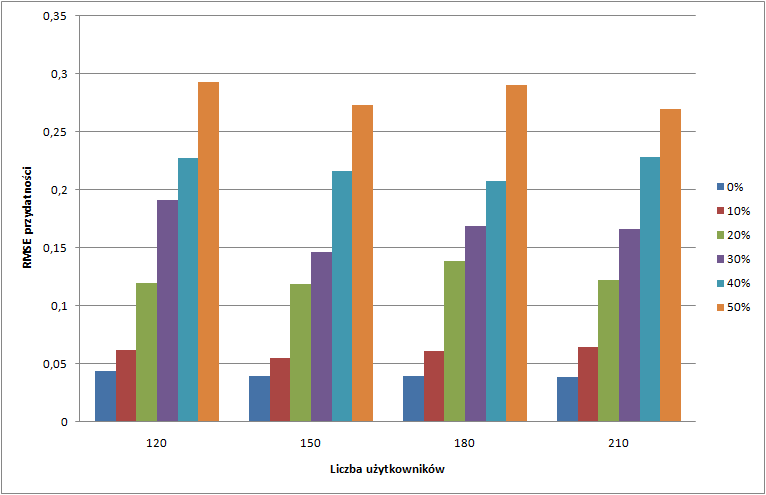
\includegraphics[width=\textwidth, keepaspectratio=true]{images/LiarsTest.png}
	\caption{Liczba użytkowników a~pierwiastek błędu średniokwadratowego przydatności recenzji}\label{fig:test3}
\end{figure}

Jak widać na powyższym wykresie, wzrost liczby oszustów w~systemie skutkuje wzrostem wartości błędu niezależnie od liczby użytkowników. Ponadto warto zauważyć, że przy dziesięcioprocentowym udziale oszustów w~systemie wartość błędu różni się nieznacznie od wartości błędu w~sytuacji gdy wszyscy użytkownicy są rzetelni.

\subsection{Testowanie z~wykorzystaniem arkusza kalkulacyjnego}

Przedstawiona poniżej tabela \ref{tab:test1} opracowana została na podstawie obliczeń wykonanych za pomocą arkusza kalkulacyjnego i~zawiera najważniejsze informacje dotyczące recenzji: liczbę oddanych głosów, liczbę głosów pozytywnych i~przydatność wyliczoną na podstawie wzoru \ref{eq:przydatnosc}. Zastosowanie arkusza kalkulacyjnego pozwoliło na manualny dobór liczby głosów, średniej systemu i~ogólnej oceny recenzenta, dzięki czemu możliwe było przetestowanie charakterystycznych przypadków. Przedstawione wyniki dotyczą systemu, w~którym średnia przydatność wynosi 50\%, a~wszyscy recenzenci mają identyczną ocenę i~liczbę otrzymanych głosów. Wartości pozostałych parametrów wynoszą odpowiednio: $C=15$, $w_{m}=1$, $w_{g}=8$, $w_{a}=3$.

\begin{table}[H]
\centering
    \begin{tabular}{|l|l|l|l|}
    \hline
    lp. & liczba głosów & liczba głosów pozytywnych & przydatność [\%] \\ \hline\hline
    1. & 1 & 1 & 71,28 \\ \hline
    2. & 3 & 3 & 78,57 \\ \hline
    3. & 5 & 5 & 82,91 \\ \hline
    4. & 9 & 9 & 87,84 \\ \hline
    5. & 15 & 15 & 91,51 \\ \hline
    6. & 20 & 20 & 93,22 \\ \hline
    7. & 3 & 0 & 40,47 \\ \hline
    8. & 5 & 0 & 32,27 \\ \hline
    9. & 10 & 0 & 21,42 \\ \hline
    \end{tabular}
	\caption{Rezultaty eksperymentu}\label{tab:test1}
\end{table}

Pozycje 1. - 6. dotyczą sytuacji, w~której wszystkie głosy oddane na recenzję są pozytywne. W tradycyjnym podejściu, znanym z~istniejących serwisów, przydatność wynosiłaby wtedy 100\%. Dzięki zastosowaniu średniej Bayesa, wartość przydatności normalizowana jest przez średnią przydatność systemu, a~istotność głosów rośnie wraz z~ich liczbą. Zatem by posiadać większą przydatność recenzja musi posiadać więcej głosów, nawet jeżeli wszystkie są pozytywne. Pozwala to uniknąć sytuacji znanej z~istniejących serwisów, gdzie jeden głos pozytywny powoduje umieszczenie produktu na szczycie rankingu.

Istotność średniej przydatności w~systemie, czyli to jak mocno oddziałuje ona na pozostałe składowe, określa się za pomocą stałej C, uwzględnionej we wzorze \ref{eq:przydatnosc} oraz dodatkowo za pomocą wag odnoszących się do poszczególnych składników.

Pozycje 7. - 9. dotyczą sytuacji, gdy wszystkie głosy oddane na recenzję są negatywne. W tym przypadku średnia Bayesa działa analogicznie, normalizując przydatność w~kierunku wartości średniej.


\section{Implementacja}

W celu implementacji algorytmu rankingowego stworzone zostały metody pozwalające obliczyć przydatność recenzji i~ocenę recenzenta, a~także metody pomocnicze obliczające ich składowe. Przydatność recenzji oraz ocena autora zrealizowane zostały jako pola, odpowiednio w~klasach Review i~User, których obiekty przechowywane są w~bazie danych. Umożliwia to przede wszystkim efektywne sortowanie danych na poziomie bazy danych. Wspomniane wartości obliczane są za każdym razem, gdy któryś z~użytkowników odda głos na recenzję. Część kliencka aplikacji rozpoczyna wtedy asynchroniczną komunikację z~serwerem i~wysyła informację o~typie głosu, identyfikatorze recenzji i~nazwie użytkownika oddającego głos. Na serwerze, dane przetwarzane są w~ramach jednej transakcji\cite{springAction}, dzięki czemu zachowana jest ich spójność. Głos zostaje skojarzony z~zalogowanym użytkownikiem i~ocenioną recenzją, a~następnie obliczana jest nowa wartość użyteczności recenzji i~rangi jej autora. Wartości te są następnie przesyłane do warstwy klienckiej i~prezentowane użytkownikowi.

Jednym z~elementów potrzebnych do obliczenia przydatności recenzji jest średnia przydatność wszystkich recenzji w~systemie. W przypadku bardzo dużej bazy danych obliczenie tej wartości byłoby czasochłonne, a~to spowodowałoby znaczny wzrost czasu odpowiedzi serwisu. Aby temu zapobiec, aktualna wartość średniej przechowywana jest w~bazie danych i~aktualizowana okresowo przy wykorzystaniu biblioteki Quartz, która umożliwia wykonywanie zadań w~określonych odstępach czasu bez interakcji z~użytkownikiem.\cite{quartz} Każdorazowe przeliczenie średniej wiąże się dodatkowo z~przeliczeniem przydatności dla każdej recenzji, tak by odzwierciedlały one aktualny stan systemu i~można było je porównywać. Oczywiście, takie rozwiązanie najlepiej sprawdza się w~przypadku gdy liczba  recenzji w~bazie jest stosunkowo duża, ponieważ można wtedy założyć, że pojedynczy głos ma bardzo mały wpływ na średnią i~jej ciągłe przeliczanie byłoby nieopłacalne.

\section{Problemy i~wnioski}

Przedstawiona koncepcja algorytmu rankingowego może być z~powodzeniem zastosowana w~komercyjnym serwisie. Dzięki zastosowaniu średniej Bayesa do obliczania przydatności, system daje użytkownikowi możliwość zaobserwowania nie tylko jak dana recenzja jest oceniana, ale także jak wypada na tle innych recenzji. Dodatkowo, w~porównaniu do konwencjonalnych rozwiązań, ranking zbudowany przy zastosowaniu proponowanej koncepcji jest bardziej wiarygodny i~odporny na manipulację przez nieuczciwych użytkowników.

Proponowane rozwiązanie niesie ze sobą także pewne problemy. Najważniejszym z~nich jest dobór stałych wykorzystywanych we wzorach na przydatność i~rangę użytkownika. Wartości te dobierane są w~oparciu o~intuicję lub eksperymentalnie, co niesie ryzyko, że wybrana ostatecznie konfiguracja okaże się nieoptymalna.
